\section{某些曲面的基本群}
\label{section:ch09-sec60}

重新提一下, 曲面是具有可数基的 Hausdorff 空间, 它的每一点有一个邻域同胚于 $\mathbb{R}^{2}$ 中某一个开子集. 许多数学分支中都研究曲面, 例如几何、拓扑、复分析等. 我们在这里只考虑几个曲面, 包括环面、双环面等, 并通过比较它们的基本群来证明它们互不同胚. 在下一章中, 我们将对所有紧致曲面进行分类.

首先, 考虑环面. 在前面的习题中, 曾经要求过读者通过覆叠空间的理论来计算它的基本群. 现在, 我们将用关于积空间基本群的定理来计算它的基本群.

回顾一下, 如果 $A$ 和 $B$ 是以"$\cdot$"为运算的群, 则用下式定义笛卡儿积 $A\times B$ 中的运算, 使得它成为一个群:
\[
(a\times b)\cdot(a'\times b')=(a\cdot a')\times(b\cdot b').
\]
此外, 如果 $h\colon C\to A$ 和 $k\colon C\to B$ 是群的同态, 则映射 $\Phi\colon C\to A\times B$ 也是群的同态, 其定义为 $\Phi(c)=h(c)\times k(c)$.

\begin{theorem}
\label{theorem:ch09-sec60-60-1}
$\pi_1(X\times Y,x_0\times y_0)$ 同构于 $\pi_1(X,x_0)\times\pi_1(Y,y_0)$.
\end{theorem}

\begin{proof}
设 $p\colon X\times Y\to X$ 和 $q\colon X\times Y\to Y$ 为投射. 如果使用定理陈述中的基点, 我们有诱导同态
\[
p_{*}\colon\pi_{1}(X\times Y,x_{0}\times y_{0})\longrightarrow\pi_{1}(X,x_{0}),\qquad
q_{*}\colon\pi_{1}(X\times Y,x_{0}\times y_{0})\longrightarrow\pi_{1}(Y,y_{0}).
\]
定义同态
\[
\Phi\colon\pi_{1}(X\times Y,x_{0}\times y_{0})\longrightarrow\pi_{1}(X,x_{0})\times\pi_{1}(Y,y_{0})
\]
使得
\[
\Phi([f])=p_{*}([f])\times q_{*}([f])=[p\circ f]\times[q\circ f].
\]
以下证明 $\Phi$ 是一个同构.

$\Phi$ 是一个满射. 设 $g\colon I\to X$ 是以 $x_0$ 为基点的一条回路, $h\colon I\to Y$ 是以 $y_0$ 为基点的一条回路. 我们来证明元素 $[g]\times[h]$ 在 $\Phi$ 的像中. 定义 $f\colon I\to X\times Y$ 使得
\[
f(s)=g(s)\times h(s).
\]
则 $f$ 是 $X\times Y$ 中以 $x_0\times y_0$ 为基点的一条回路, 并且
\[
\Phi([f])=[p\circ f]\times[q\circ f]=[g]\times[h],
\]
这正是我们要证明的.

$\Phi$ 的核是蜕化的. 设 $f\colon I\to X\times Y$ 是 $X\times Y$ 中以 $x_0\times y_0$ 为基点的一条回路, 使得 $\Phi([f])=[p\circ f]\times[q\circ f]$ 是单位元. 这意味着 $p\circ f\simeq_p e_{x_0}$ 和 $q\circ f\simeq_p e_{y_0}$. 设 $G$ 和 $H$ 分别是它们的道路同伦. 这时, 映射 $F\colon I\times I\to X\times Y$ 便是 $f$ 与以 $x_0\times y_0$ 为基点的常值映射之间的道路同伦, 定义为
\[
F(s,t)=G(s,t)\times H(s,t).
\]
\end{proof}

\par
\begin{figure}[htbp]
\centering
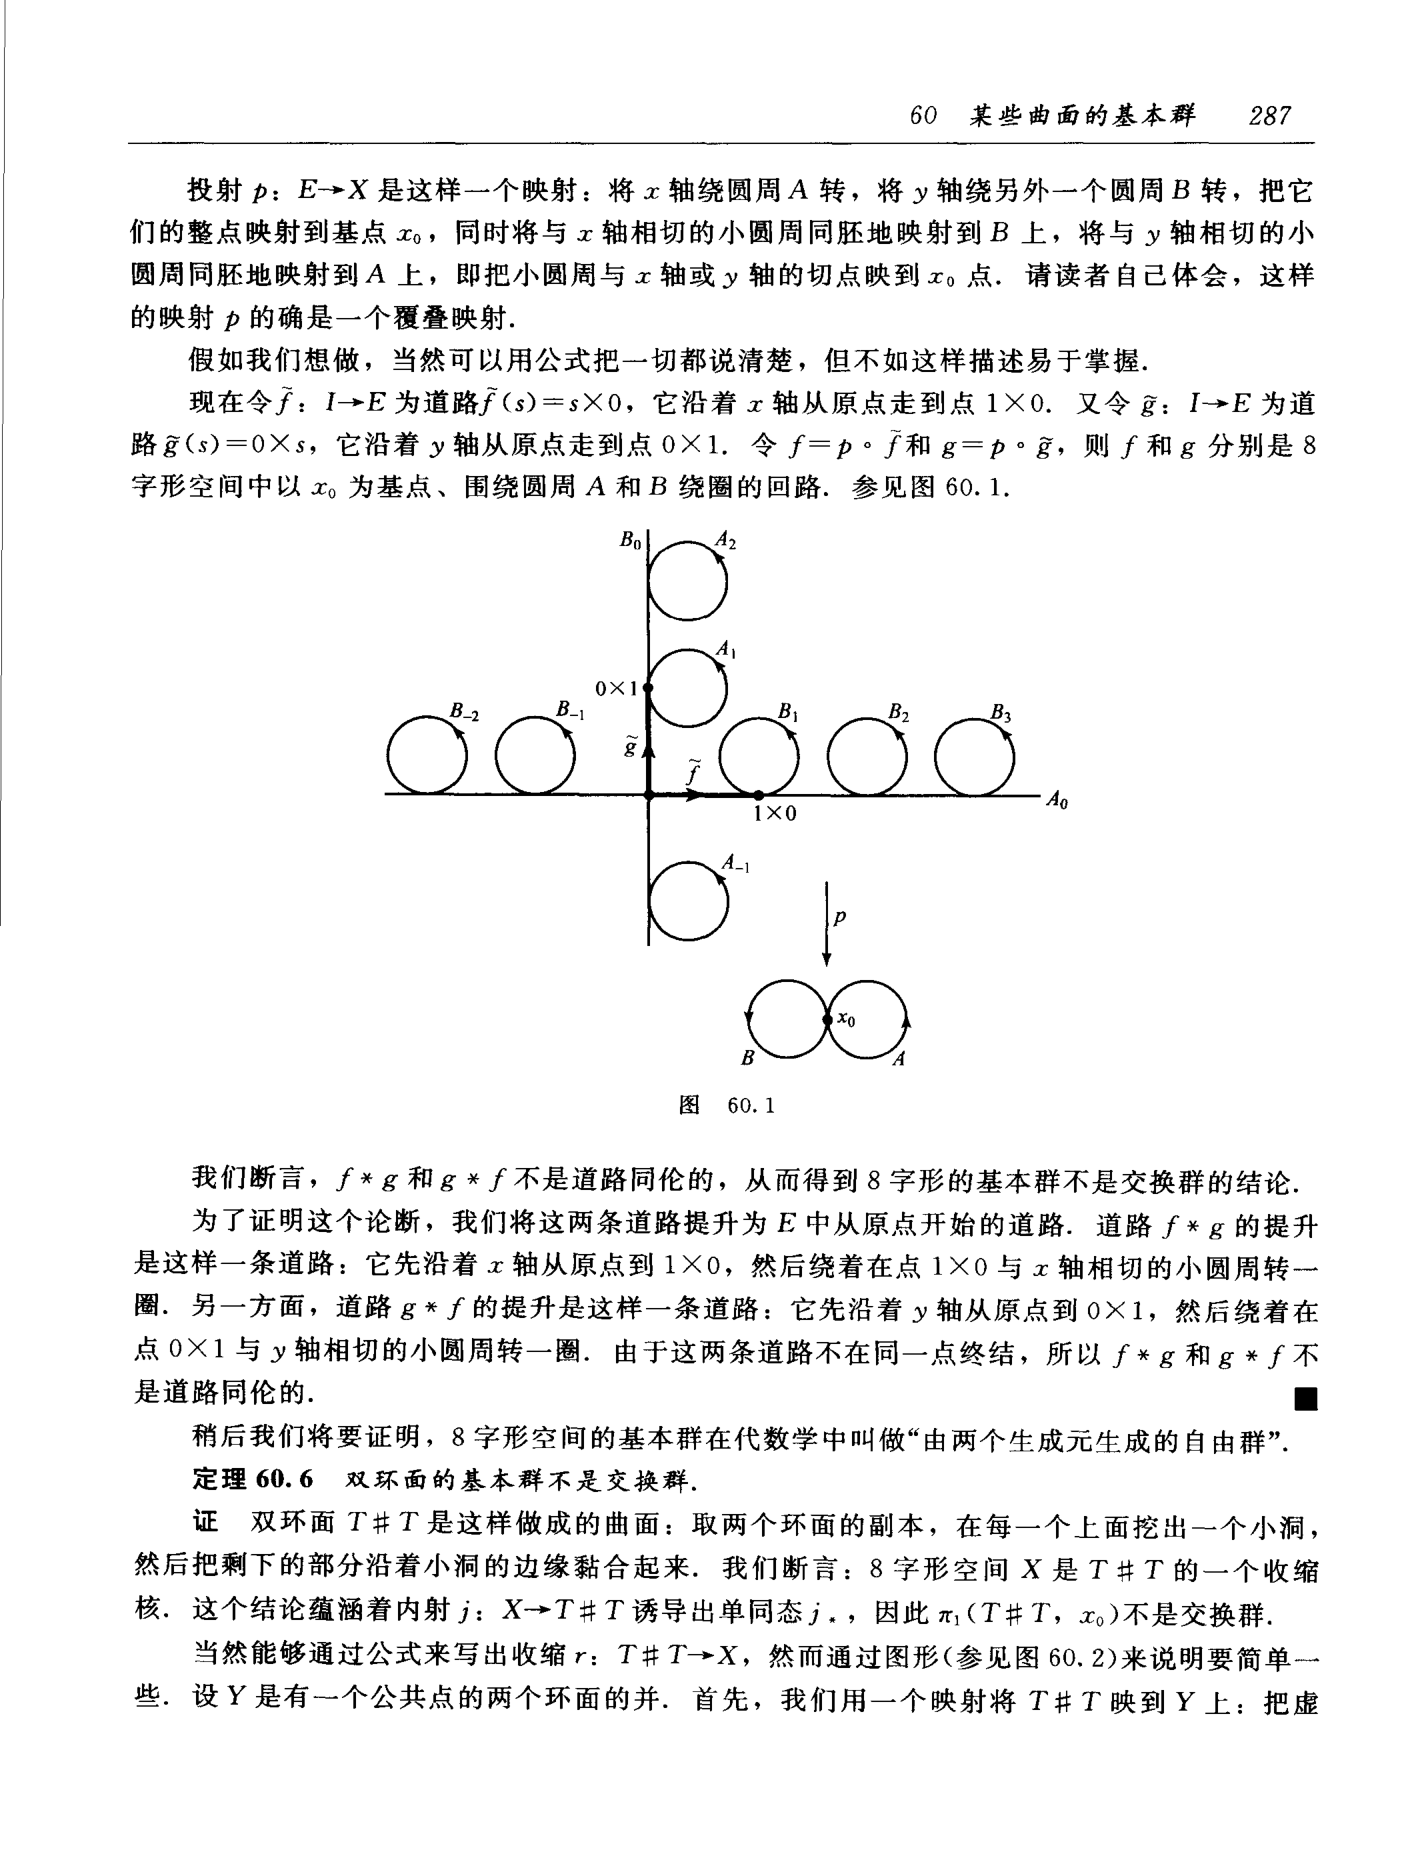
\includegraphics[width=0.7\textwidth]{image/fig-60-1.png}
\caption{8 字形空间的覆叠空间.}
\label{figure:ch09-fig-60-1}
\end{figure}

\par
\begin{figure}[htbp]
\centering
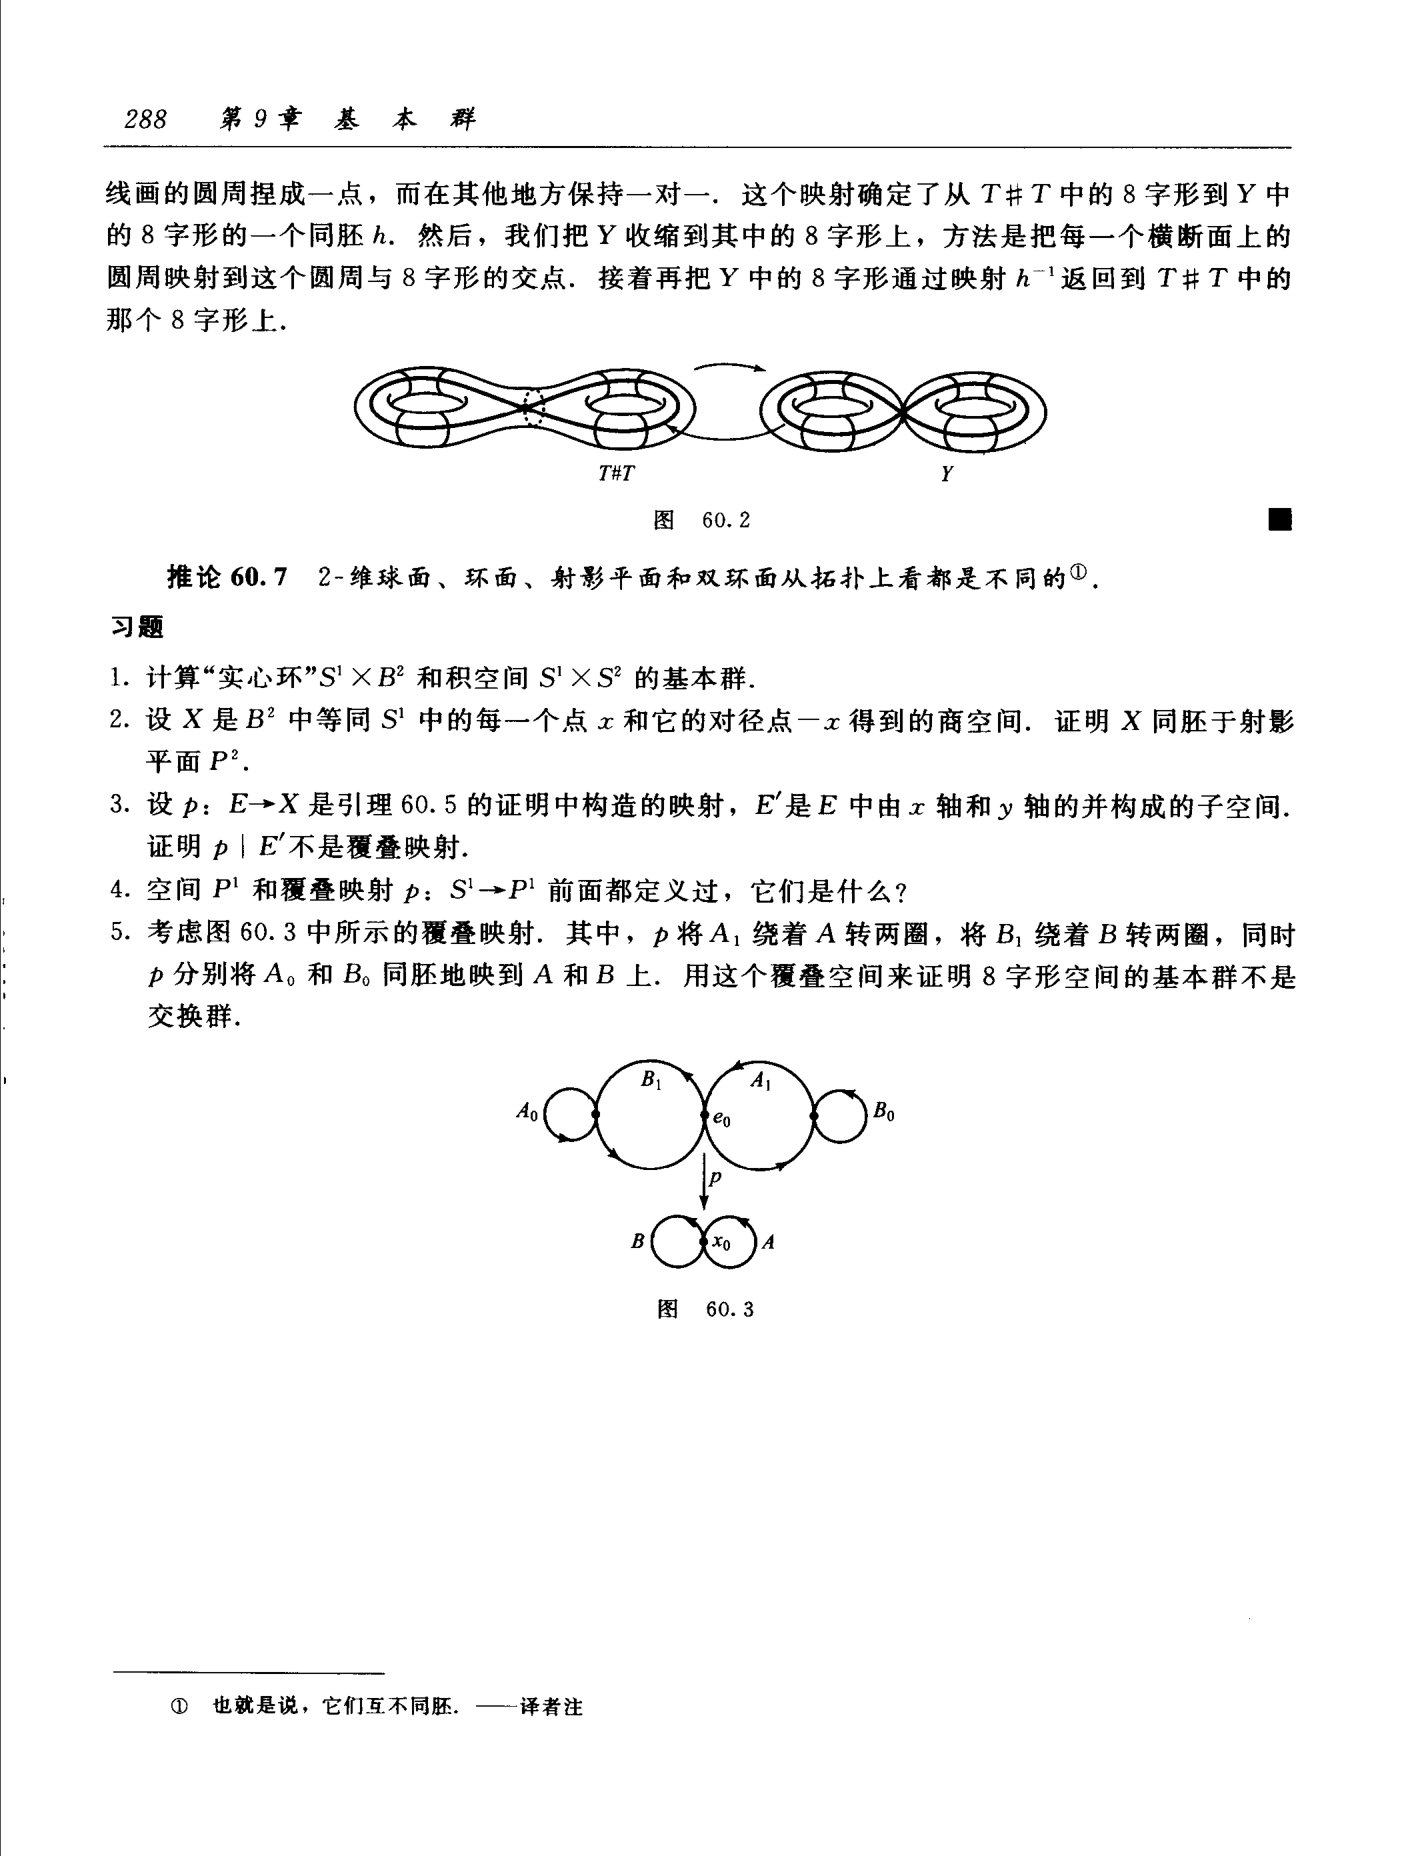
\includegraphics[width=0.7\textwidth]{image/fig-60-2.png}
\caption{双环面收缩到 8 字形空间.}
\label{figure:ch09-fig-60-2}
\end{figure}

\par
\begin{figure}[htbp]
\centering
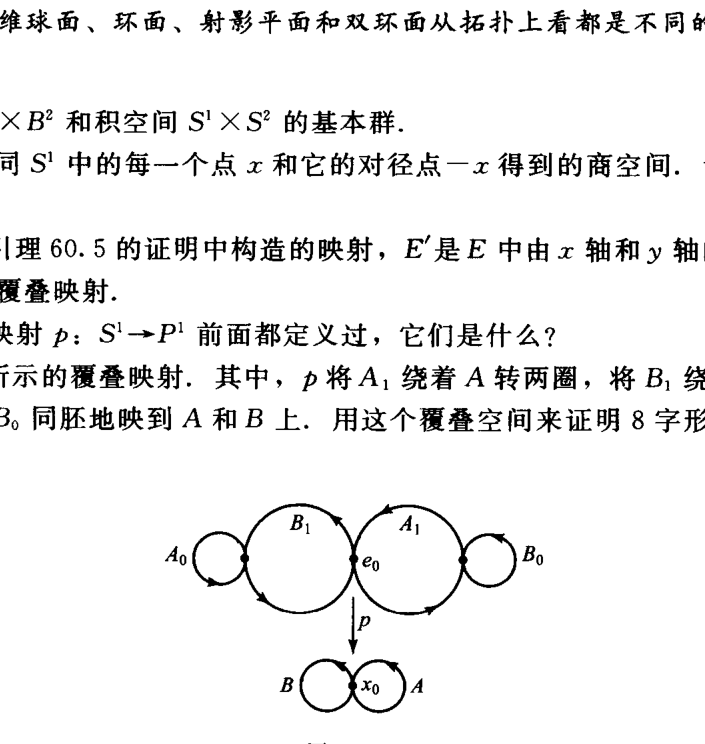
\includegraphics[width=0.5\textwidth]{image/fig-60-3.png}
\caption{习题 5.}
\label{figure:ch09-fig-60-3}
\end{figure}

\begin{corollary}
\label{corollary:ch09-sec60-60-2}
环面 $T=S^{1}\times S^{1}$ 的基本群同构于群 $\mathbb{Z}\times\mathbb{Z}$.
\end{corollary}

现在来定义一个叫做射影平面的曲面并且计算它的基本群.

\begin{definition}[射影平面]
\label{definition:ch09-sec60-projective}
\textbf{射影平面}(projective plane) $P^{2}$ 是 $S^{2}$ 中等同每一个点 $x$ 与它的对径点 $-x$ 而得到的商空间.
\end{definition}

射影平面不是一个读者所熟悉的空间, 不能嵌入到 $\mathbb{R}^{3}$ 中, 也难于直观. 然而它是射影几何所研究的基本对象, 就像欧氏空间 $\mathbb{R}^{2}$ 对于通常的欧氏几何一样. 拓扑学家的兴趣所在是将它作为曲面的例子.

\begin{theorem}
\label{theorem:ch09-sec60-60-3}
射影平面 $P^{2}$ 是紧致曲面, 并且商映射 $p\colon S^{2}\to P^{2}$ 是覆叠映射.
\end{theorem}




\begin{proof}
先指出 $p$ 是开映射. 设 $U$ 是 $S^{2}$ 的一个开集. 对径映射 $a\colon S^{2}\to S^{2}$, 是一个同胚其定义为 $a(x)=-x$. 因此 $a(U)$ 是 $S^{2}$ 中的一个开集. 由于集合
\[
p^{-1}(p(U))=U\cup a(U)
\]
也是 $S^{2}$ 中的开集, 因此根据定义 $p(U)$ 是 $P^{2}$ 中的开集. 类似的证明指出 $p$ 也是闭映射.

下面证明 $p$ 是覆叠映射. 给定 $P^{2}$ 中的点 $y$, 选取 $x\in p^{-1}(y)$. 对于某 $\varepsilon<1$, 选取 $x$ 在 $S^{2}$ 中的一个 $\varepsilon$-邻域 (使用 $\mathbb{R}^{3}$ 中的欧氏度量 $d$). $U$ 不会包含 $S^{2}$ 的任何一对对径点 $\{z,a(z)\}$, 这是因为 $d(z,a(z))=2$. 从而映射
\[
p\colon U\longrightarrow p(U)
\]
是一一的. 由于它是连续的开映射, 所以它是一个同胚. 类似地,
\[
p\colon a(U)\longrightarrow p(a(U))=p(U)
\]
也是一个同胚. 于是集合 $p^{-1}(p(U))$ 便是无交的开集 $U$ 和 $a(U)$ 之并, 其中每一个都被 $p$ 同胚地映射到 $p(U)$. 因此 $p(U)$ 是 $p(x)=y$ 被 $p$ 均衡地覆盖着的邻域.

由于 $S^{2}$ 有可数基 $\{U_n\}$, 所以空间 $P^{2}$ 有可数基 $\{p(U_n)\}$.

$P^{2}$ 是一个 Hausdorff 空间是因为 $S^{2}$ 是正规空间并且 $p$ 是闭映射. (见第 31 节中的习题 6.) 我们还可以给出一个另外的直接证明如下: 设 $y_1$ 和 $y_2$ 是 $P^{2}$ 中的两个点. 集合 $p^{-1}(y_1)\cup p^{-1}(y_2)$ 由四个点组成. 设 $2\varepsilon$ 为这四个点中每两个点的距离的最小者. 令 $U_1$ 为 $p^{-1}(y_1)$ 中的某一个点的 $\varepsilon$-邻域, $U_2$ 为 $p^{-1}(y_2)$ 中的某一个点的 $\varepsilon$-邻域, 则
\[
U_{1}\cup a(U_{1})\quad\text{和}\quad U_{2}\cup a(U_{2})
\]
是无交的. 这蕴涵着 $p(U_1)$ 和 $p(U_2)$ 分别是 $y_1$ 和 $y_2$ 在 $P^{2}$ 中的无交邻域.

由于 $S^{2}$ 是一个曲面并且 $P^{2}$ 的每一个点有一个邻域同胚于 $S^{2}$ 中的某一个开子集, 所以空间 $P^{2}$ 也是一个曲面.
\end{proof}

\begin{corollary}
\label{corollary:ch09-sec60-60-4}
$\pi_1(P^{2},y)$ 是一个 $2$ 阶群.
\end{corollary}

\begin{proof}
投射 $p\colon S^{2}\to P^{2}$ 是一个覆叠映射. 由于 $S^{2}$ 是单连通的, 应用定理 \cref{theorem:ch09-sec54-54-4} 可见, 在 $\pi_1(P^{2},y)$ 与集合 $p^{-1}(y)$ 之间有一个一一对应. 由于后者是一个二元素集, 所以 $\pi_1(P^{2},y)$ 是 $2$ 阶群.

任何 $2$ 阶群都同胚于整数模 $2$ 群 $\mathbb{Z}/2$.
\end{proof}

对于任意 $n\in\mathbb{Z}_{+}$, 可以类似地将 $P^{n}$ 定义为在 $S^{n}$ 中等同每一个点 $x$ 与它的对径点 $-x$ 而得到的商空间, 并称之为 $n$ 维射影空间. 定理 \cref{theorem:ch09-sec60-60-3} 的证明不用作任何改变便可以用于证明投射 $p\colon S^{n}\to P^{n}$ 是覆叠映射. 然后, 由于当 $n\geqslant 2$ 时 $S^{n}$ 是单连通的, 进而指出当 $n\geqslant 2$ 时, $\pi_1(P^{n},y)$ 是由两个元素组成的群. 请你自己考虑, 当 $n=1$ 时会发生怎样的情况.

我们现在来研究双环面, 从有关 8 字形的一个引理开始.

\begin{lemma}
\label{lemma:ch09-sec60-60-5}
8 字形的基本群不是交换群.
\end{lemma}

\begin{proof}
设 $X$ 为 $\mathbb{R}^{2}$ 中两个相交于一点 $x_0$ 的圆周 $A$ 与 $B$ 的并. 我们来描述 $X$ 的一个覆叠空间 $E$.

空间 $E$ 为 $\mathbb{R}^{2}$ 的子空间, 由以下几部分组成: $x$ 轴, $y$ 轴, 在 $x$ 轴的每一个非整点上与 $x$ 轴相切的一个小圆周, 以及在 $y$ 轴的每一个非整点上与 $y$ 轴相切的一个小圆周.

投射 $p\colon E\to X$ 是这样一个映射: 将 $x$ 轴绕圆周 $A$ 转, 将 $y$ 轴绕另外一个圆周 $B$ 转, 把它们的整点映射到基点 $x_0$, 同时将与 $x$ 轴相切的小圆周同胚地映射到 $B$ 上, 将与 $y$ 轴相切的小圆周同胚地映射到 $A$ 上, 即把小圆周与 $x$ 轴或 $y$ 轴的切点映到 $x_0$ 点. 请读者自己体会, 这样的映射 $p$ 的确是一个覆叠映射.

假如我们想做, 当然可以用公式把一切都说清楚, 但不如这样描述易于掌握.

现在令 $\tilde{f}\colon I\to E$ 为道路 $\tilde{f}(s)=s\times 0$, 它沿着 $x$ 轴从原点走到点 $1\times 0$. 又令 $\tilde{g}\colon I\to E$ 为道路 $\tilde{g}(s)=0\times s$, 它沿着 $y$ 轴从原点走到 $0\times 1$. 令 $f=p\circ\tilde{f}$ 和 $g=p\circ\tilde{g}$, 则 $f$ 和 $g$ 分别是 8 字形空间中以 $x_0$ 为基点、围绕圆周 $A$ 和 $B$ 绕圈的回路. 参见图 \cref{figure:ch09-fig-60-1}.


我们断言, $f*g$ 和 $g*f$ 不是道路同伦的, 从而得到 8 字形的基本群不是交换群的结论.

为了证明这个论断, 我们将这两条道路提升为 $E$ 中从原点开始的道路. 道路 $f*g$ 的提升是这样一条道路: 它先沿着 $x$ 轴从原点到 $1\times 0$, 然后绕着在点 $1\times 0$ 与 $x$ 轴相切的小圆周转一圈. 另一方面, 道路 $g*f$ 的提升是这样一条道路: 它先沿着 $y$ 轴从原点到 $0\times 1$, 然后绕着在点 $0\times 1$ 与 $y$ 轴相切的小圆周转一圈. 由于这两条道路不在同一点终结, 所以 $f*g$ 和 $g*f$ 不是道路同伦的.
\end{proof}

稍后我们将要证明, 8 字形空间的基本群在代数学中叫做"由两个生成元生成的自由群".

\begin{theorem}
\label{theorem:ch09-sec60-60-6}
双环面的基本群不是交换群.
\end{theorem}

\begin{proof}
双环面 $T\# T$ 是这样做成的曲面: 取两个环面的副本, 在每一个上面挖出一个小洞, 然后把剩下的部分沿着小洞的边缘黏合起来. 我们断言: 8 字形空间 $X$ 是 $T\# T$ 的一个收缩核. 这个结论蕴涵着内射 $j\colon X\to T\# T$ 诱导出单同态 $j_*$, 因此 $\pi_1(T\# T,x_0)$ 不是交换群.

当然能够通过公式来写出收缩 $r\colon T\# T\to X$, 然而通过图形 (参见图 \cref{figure:ch09-fig-60-2}) 来说明要简单一些. 设 $Y$ 是有一个公共点的两个环面的并. 首先, 我们用一个映射将 $T\# T$ 映到 $Y$ 上: 把虚线画的圆周捏成一点, 而在其他地方保持一对一. 这个映射确定了从 $T\# T$ 中的 8 字形到 $Y$ 中的 8 字形的一个同胚 $h$. 然后, 我们把 $Y$ 收缩到其中的 8 字形上, 方法是把每一个横断面上的圆周映射到这个圆周与 8 字形的交点. 接着再把 $Y$ 中的 8 字形通过映射 $h^{-1}$ 返回到 $T\# T$ 中的那个 8 字形上.
\end{proof}


\begin{corollary}
\label{corollary:ch09-sec60-60-7}
$2$-维球面、环面、射影平面和双环面从拓扑上看都是不同的.
\end{corollary}

\subsection*{习题}

\begin{exercise}
计算"实心环" $S^{1}\times B^{2}$ 和积空间 $S^{1}\times S^{2}$ 的基本群.
\end{exercise}

\begin{exercise}
设 $X$ 是 $B^{2}$ 中等同 $S^{1}$ 中的每一个点 $x$ 和它的对径点 $-x$ 得到的商空间. 证明 $X$ 同胚于射影平面 $P^{2}$.
\end{exercise}

\begin{exercise}
设 $p\colon E\to X$ 是引理 \cref{lemma:ch09-sec60-60-5} 的证明中构造的映射, $E'$ 是 $E$ 中由 $x$ 轴和 $y$ 轴的并构成的子空间. 证明 $p\mid E'$ 不是覆叠映射.
\end{exercise}

\begin{exercise}
空间 $P^{1}$ 和覆叠映射 $p\colon S^{1}\to P^{1}$ 前面都定义过, 它们是什么?
\end{exercise}

\begin{exercise}
考虑图 \cref{figure:ch09-fig-60-3} 中所示的覆叠映射. 其中, $p$ 将 $A_1$ 绕着 $A$ 转两圈, 将 $B_1$ 绕着 $B$ 转两圈, 同时 $p$ 分别将 $A_0$ 和 $B_0$ 同胚地映到 $A$ 和 $B$ 上. 用这个覆叠空间来证明 8 字形空间的基本群不是交换群.
\end{exercise}